\section{Case Study}
\label{sec:simulation}

Figure~\ref{fig:simulation} depicts the behavior of a UAV, modeled as a
planar-vehicle behaves under the control strategy devised in
Section~\ref{sec:control}. As the gradient vector field $\nabla_qV(q) \rightarrow
0$ as the distance of the UAV to one of the wires goes to zero, the vehicle only
asymptotically reaches the wire, gradually coming to rest as it approaches the
wire.
%
\begin{figure}[tbh]
  \centering
  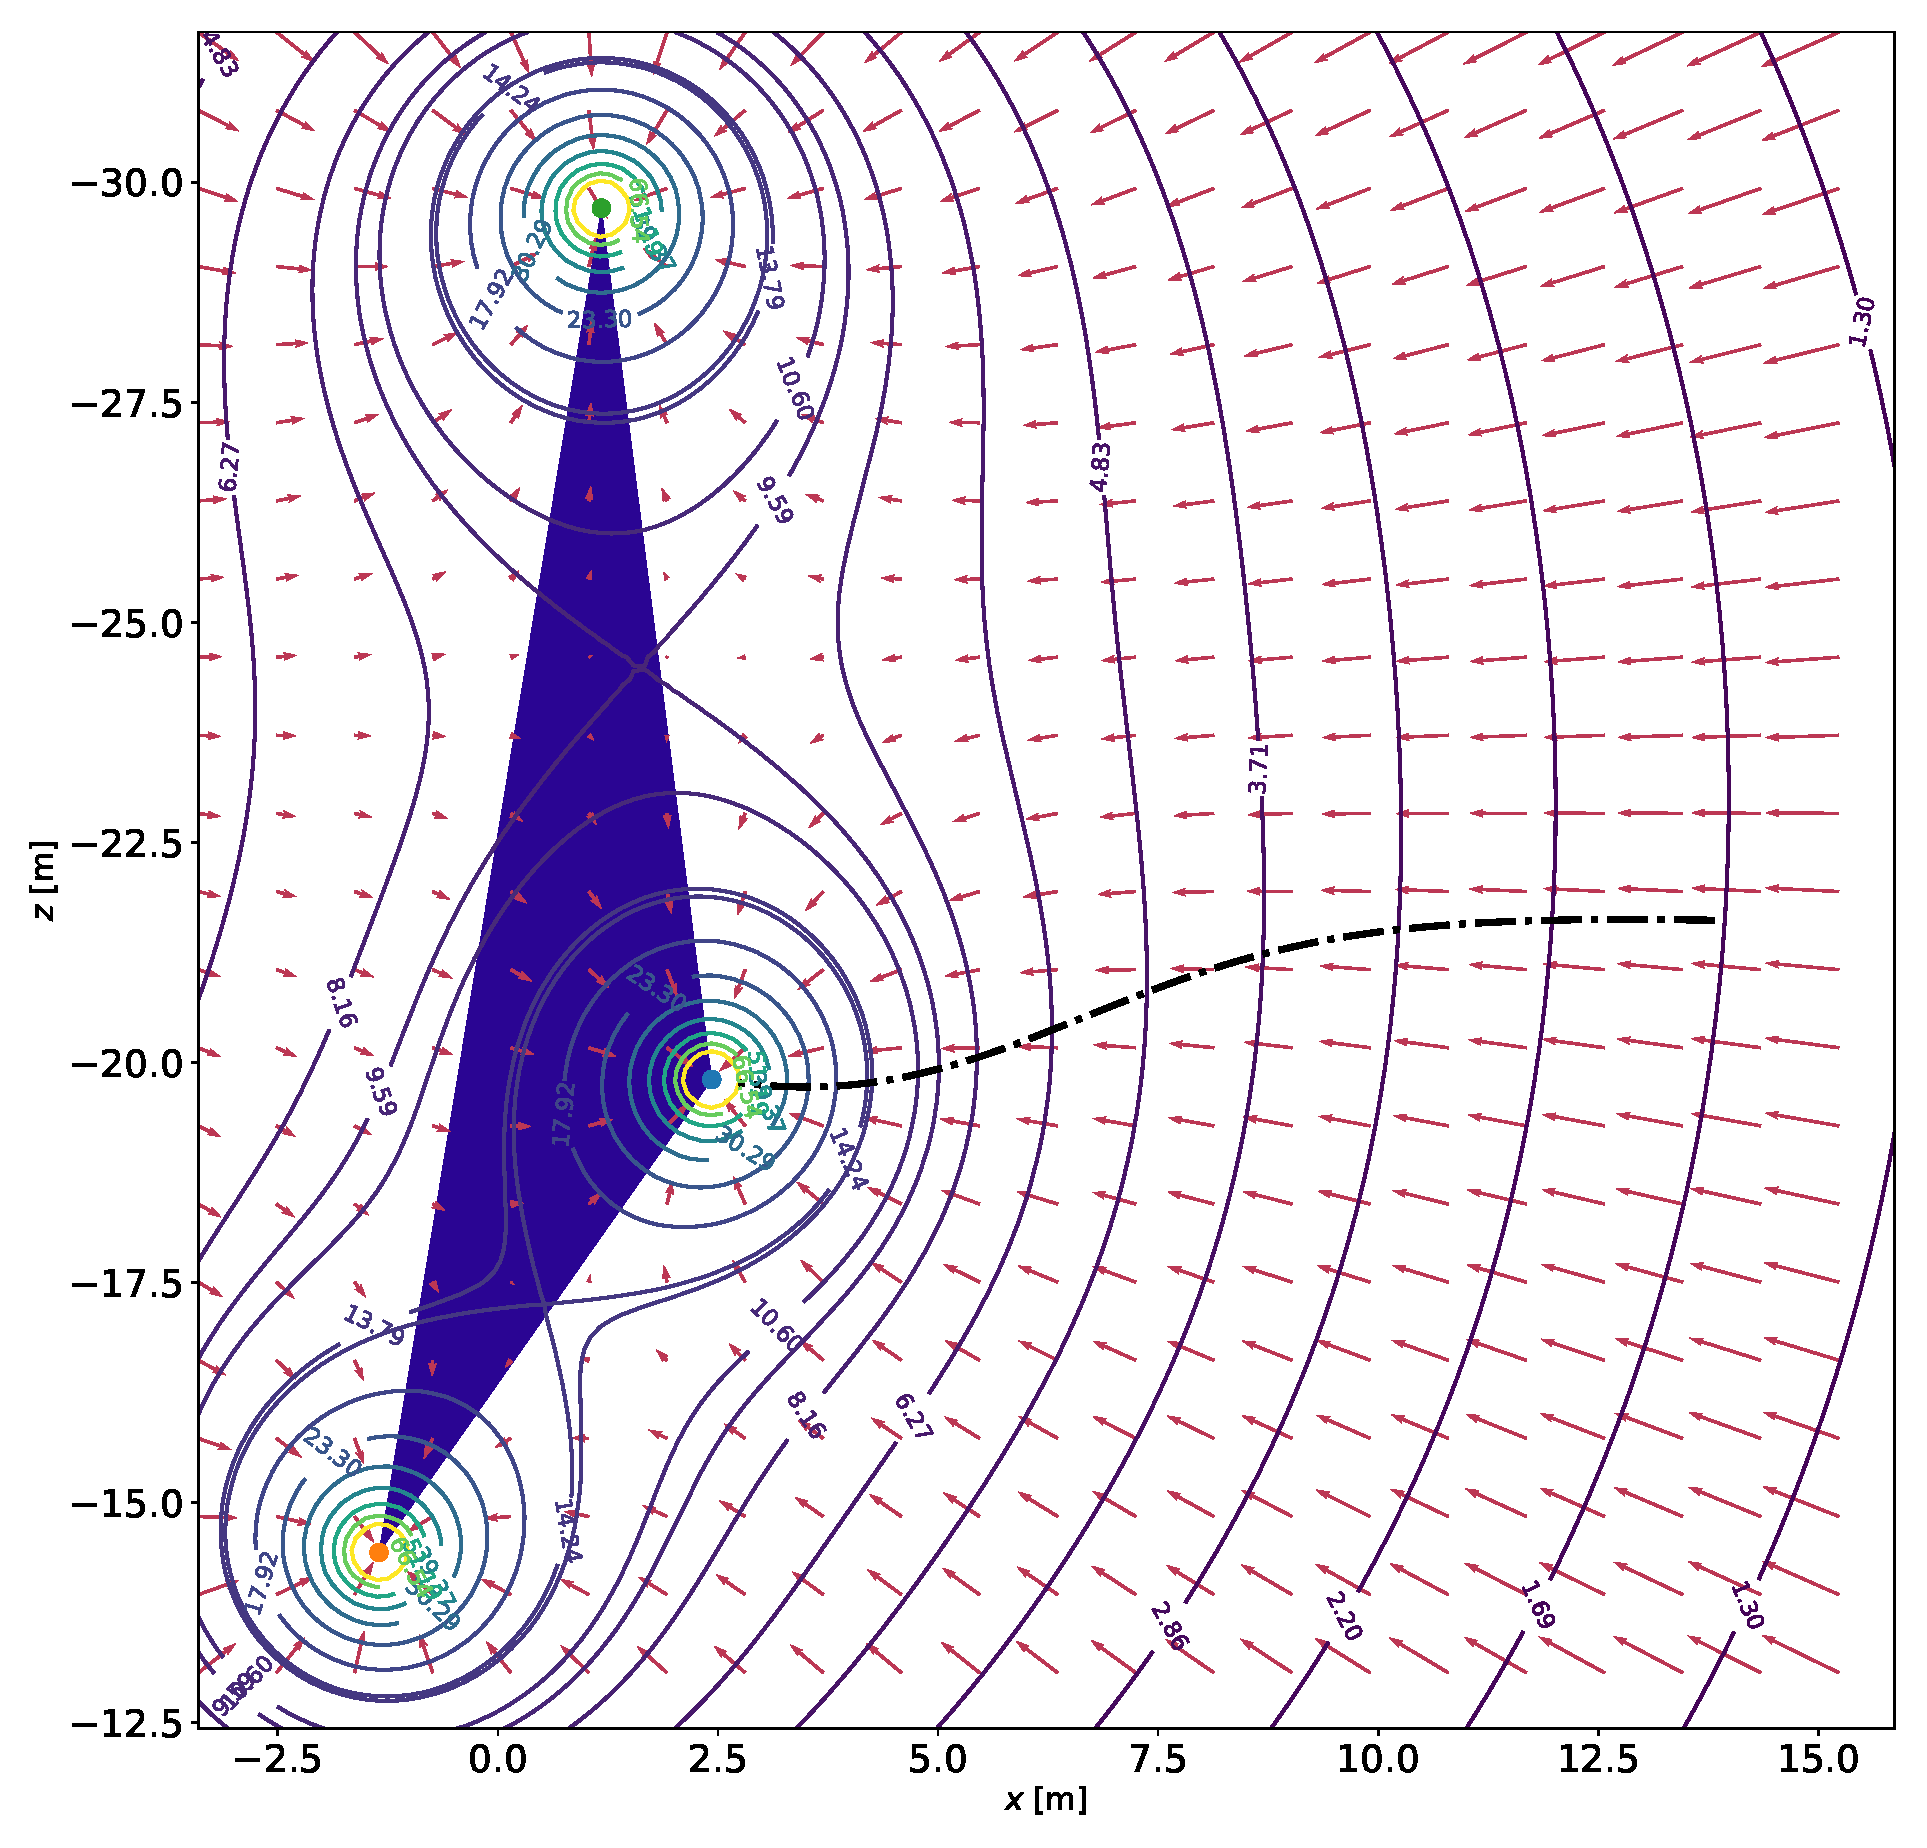
\includegraphics[width=0.45\textwidth]{./figures/simtraj.eps}
  \caption{Sample trajectory of a UAV under the control strategy provided in
  Section~\ref{sec:control}. The dash-dotted black line depicts the motion of
    the UAV in the $(x,z)$-plane.}
  \label{fig:simulation}
\end{figure}
%
